%%%%%%%%%%%%%%%%
\section{Simulation Validation}
\label{sec:SimValidation}

\subsection{Energy Deposition Validaiton}
The energy deposition was tested by reproducing the single collision energy loss spectra in water\footnote{%
An analyis class was not written for this simulation. 
Instead the verbosity of the simulation was set to \verb+vebose=1+ in the run macro.
The first ionisation collision (\verb+e-_G4DNAIonisation+) was then extracted with \verb+sed -n '/ParentID = 0/,/e-_G4DNAIonisation/p' G4OutputFileName.txt+ \verb+grep+ and \verb+awk+ were then used to extract the actual energy, \verb+| grep "e-\_G4DNAIonisatioin" | awk '${print $5}'+ %
}.
The \verb+PhysicsList+ was extended to include \verb+G4DNAPhysics+ and the detector material was set to the NIST defination contained in the toolkit with \verb+G4Material* H20 = man->FindOrBuildMaterial("G4_WATER")+.
In general there was excellent agreement between the simulated energy spectra and that of \cite{turner}.
The simulated spectra had much better resolution at fine energies (corresponding to discrete states) of which Turners did not.
%%%%%%%%%%%%%%%%%%%% Figures %%%%%%%%%%%%%%%%%%%%%%%%
\begin{figure}
    \centering
    \caption{Single Collision Energy Loss of Water}
    \begin{subfigure}[b]{0.45\figurewidth}
        \includegraphics[width=\textwidth]{SingleCollisionEnergyLoss_300bins}
        \caption{Simulated}
    \end{subfigure}
    \begin{subfigure}[b]{0.45\figurewidth}
        \missingfigure{Turner Fig of EDep}
        \caption{Turner}
    \end{subfigure}
\end{figure}
\subsection{Spectra Validaiton}
The simulation was validated by computing the weighted average of the energy deposition \ref{eq:AvgEnergyDepDefination} and comparing it to the spectra average defined in \ref{eq:AvgChannelNumberDefination}.
%%%%%%%%%%%%%%%%%%%%% Equations %%%%%%%%%%%%%%%%%%%%%%
\begin{equation}
\label{eq:AvgEnergyDepDefination}
<E> = \frac{\int_0^\infty {\phi(E)EdE}}{\int_0^\infty{\phi(E)dE}} \\
\text{where}
\end{equation}
\begin{equation}
\label{eq:AvgChannelNumberDefination}
<\mu> = \frac{\int_0^\infty {f(x)xdx}}{\int_0^\infty{x(x)dx}} \\
\text{where}
\end{equation}
%%%%%%%%%%%%%%%%%%%% Figures %%%%%%%%%%%%%%%%%%%%%%%%
\begin{figure}
    \centering
    \caption{Gamma Simulation Agreement}
    \includegraphics[width=\textwidth]{G4EDep_LightYield_Co60}
    \label{fig:GammaSimAgreement}
\end{figure}
\begin{figure}
    \centering
    \caption{Neutron Simulation Agreement}
    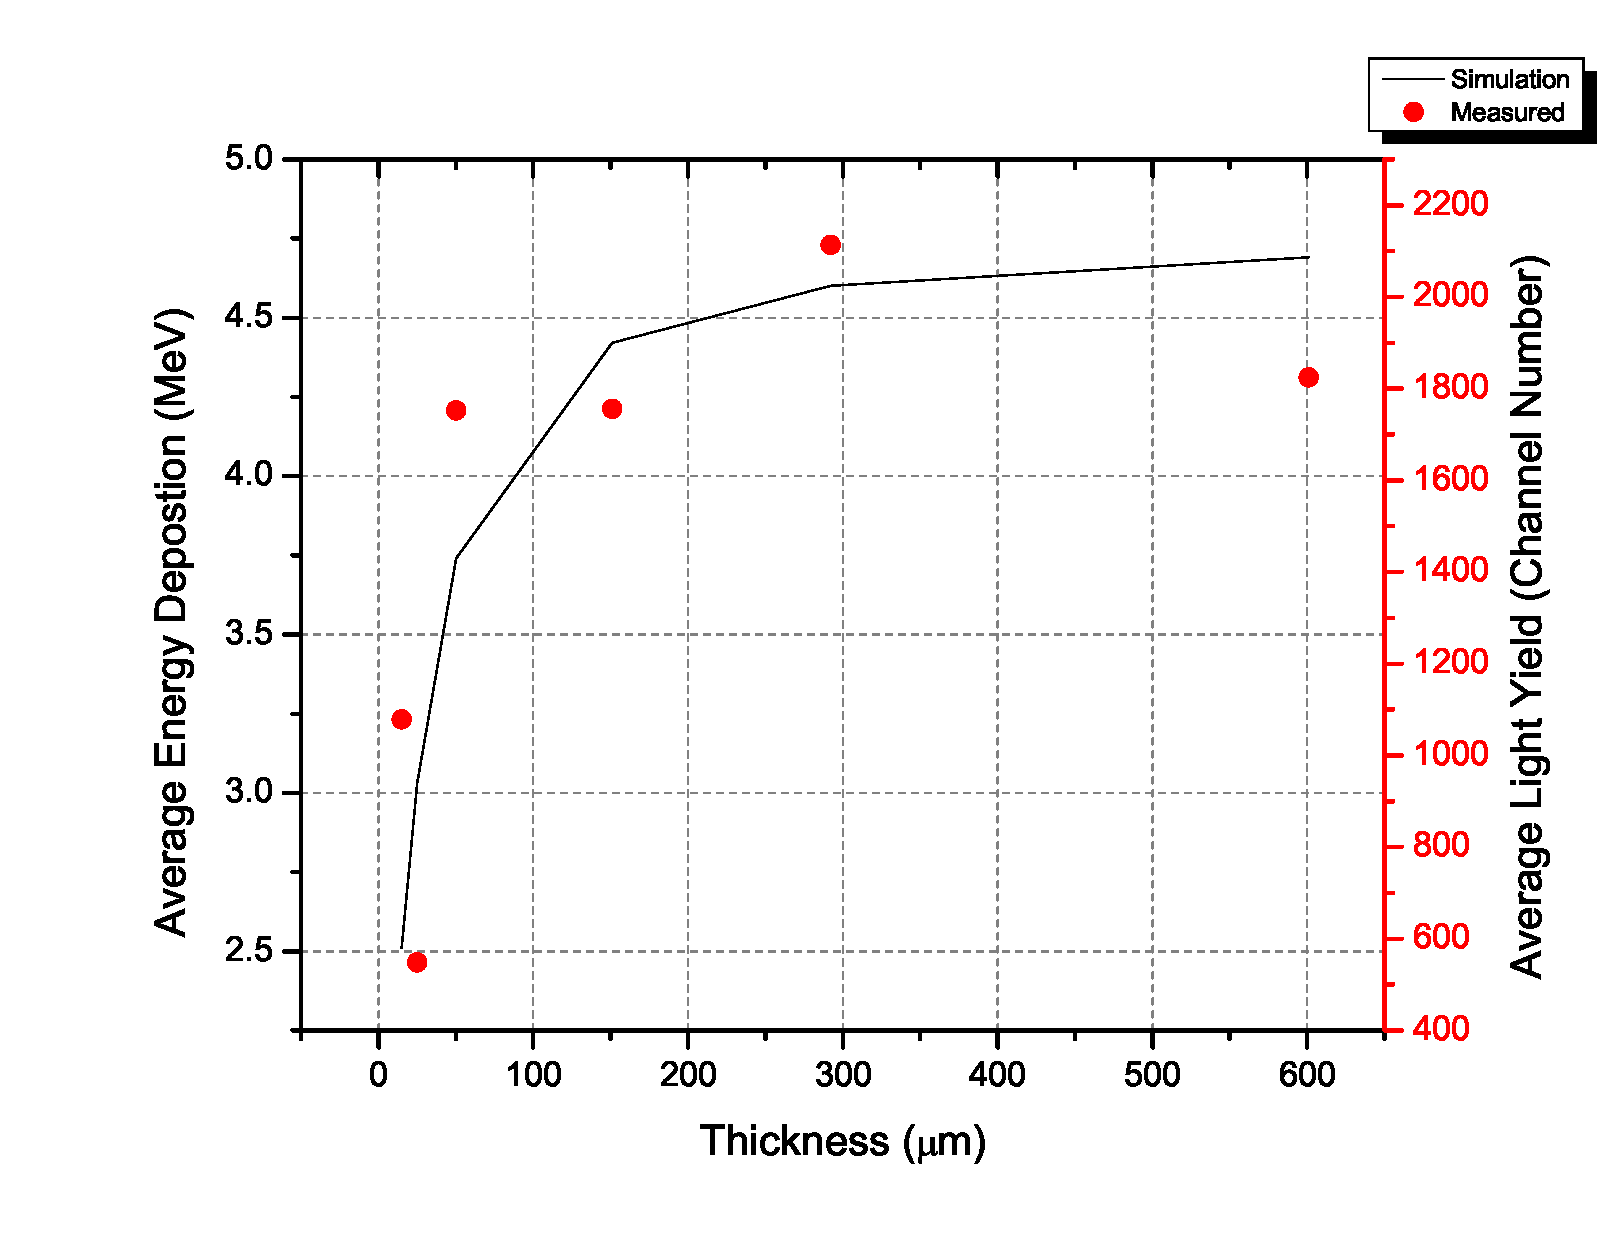
\includegraphics[width=\textwidth]{G4EDep_LightYield_Neutron}
    \label{fig:NeutronSimAgreement}
\end{figure}

